%\section{Limits of Functions}\label{limits}
\vspace{-0.25 in} %eliminate white space between chapter label and content
%%%Objectives%%%%
\begin{framed}
\subsection*{Objectives}
\begin{itemize}
    \item Using correct notation, describe the limit of a function.
    \item Be able to determine one-sided limits using a table, a graph, or a formula.
    \item Be able to determine if the limit of a function exists, and if so, determine the limiting value using a table, a graph, or a formula.
    \item Be able to algebraically find limits of polynomial and rational functions by substitution .
    \item Be able to determine limits at infinity using a table, a graph, or a formula.
    \item Determine continuity at a point on the graph of a function.
\end{itemize}

%%%Reading Assignment%%%
\subsection*{Suggested Reading:}
\begin{itemize}
\item \cite{Calaway}\footnotemark[1]
    \begin{itemize}
        \item \emph{Limits and One-Sided Limits} in Lesson 1 of Chapter 1 (pages 73-77)
        
    \end{itemize}

\item \cite{openstax}\footnotemark[2]
    \begin{itemize}
        \item \emph{Section 2.2. The Limit of a Function}\footnotemark[3]
    \end{itemize}
\item \cite{Hoffman}\footnotemark[4]
    \begin{itemize}
        \item \emph{Section 1.3: Continuous Functions}  (pages 98-103)\footnotemark[3]
        \begin{itemize}
            \item Definition and Meaning of Continuous (page 98).
            \item Why do we care whether a function is continuous? (page 101)
            \item Which Functions Are Continuous? (page 102)
        \end{itemize}
        
    \end{itemize}

\end{itemize}

%\subsection*{Supplemental Materials:}
%%%Key Terms%%%
\subsection*{Key Terms:}

\begin{multicols}{2}
\begin{itemize}
    \item Limit of a function
    \item Limit Theorems
    \item ``$x\rightarrow a$'' or ``$x$ approaches $a$"
    \item ``arbitrarily close''
\end{itemize}

\end{multicols}
%\noindent\makebox[\linewidth]{\rule{\textwidth}{0.8pt}}
\end{framed}
\footnotetext[1]{Available free to download from \url{http://www.opentextbookstore.com/details.php?id=14} .}
\footnotetext[2]{Available free to download from \url{https://openstax.org/details/books/calculus-volume-1} .}
\footnotetext[3]{Disregard any examples with trigonometry.}
\footnotetext[4]{Available free to download from \url{https://www.opentextbookstore.com/details.php?id=11#tabs-3} .}
%%%Content%%%
\newpage
\Opensolutionfile{ans}[ans1]
\Opensolutionfile{ansL}[ansL1]
%%%%%%%%%%%Idea and Notation%%%%%%%%%%%%%
\subsection*{Idea and Notation}
\hfill
\vspace{-0.5in}
\begin{wrapfigure}[13]{l}{0.4\textwidth}

\begin{figure}[H]
\captionsetup[figure]{labelsep=space}
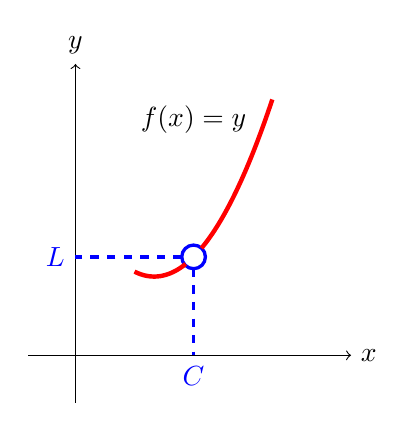
\begin{tikzpicture}[scale =1.0]
\draw[->] (-0.6,0) -- (3.5,0) node[right]{$x$};
\draw[->] (0,-0.6) -- (0,3.7) node[above]{$y$};
\draw[blue, very thick]  (1.5,1.25) circle[radius=.15];
\node at (1.5,3.0) {$f(x)=y$};
\draw[blue, very thick, dashed] (1.5,1.1)--(1.5,0)  node[below]{$C$};
\draw[blue, very thick, dashed] (1.35,1.25)--(0,1.25) node[left]{$L$};
\draw[domain=.75:1.4, smooth, variable=\x, red, ultra thick] plot ({\x}, {(\x)^2 - 2*\x +2});
\draw[domain=1.6:2.5, smooth, variable=\x, red, ultra thick] plot ({\x}, {(\x)^2 - 2*\x +2});

\end{tikzpicture}
\caption{}
\label{fig:introLimit}
\end{figure}

\end{wrapfigure}

\noindent The concept of the \textbf{limit of a function} shows up in many areas in mathematics, and it is one of the fundamental concepts in calculus.  The limit of a function describes the behavior of the function when the variable is near, but does not equal , a specified number (Figure \ref{fig:introLimit}). If the values of $f(x)$ gets closer and closer, as close as we want, to one number $L$ as we take values of $x$ very close to (but not equal to) a number $c$, then we \emph{say} \textbf{``the limit of \(f(x)\), as $\bm{x}$ approaches $\bm{c}$, is $\bm{L}$" and we \emph{write} ``\(\bm{\lim\limits_{x \to c} f(x)=L}\)" (The symbol ``\(\bm{\rightarrow}\)" means ``approaches" or "gets very close to")}.\\
\begin{spacing}{2}
\begin{tcolorbox}

\(\bm{f(c)}\) is a single number that describes the behavior (value) of \(f\) \textbf{AT} the point \(x=c\).

\(\bm{\displaystyle\lim\limits_{x \to c} f(x)}\) is a single number that describes the behavior of \(f\) \textbf{NEAR, BUT NOT AT}, the point \(x=c\).
\end{tcolorbox}
\end{spacing}
\vspace{-0.25in}
%%%%%%%%%%%Idea and Notation%%%%%%%%%%%%%

%%%%%%Alternative option from Dave's handout%%%%%%%
\begin{comment}
In terms of vocabulary, we will discuss what is meant by phrases such as:  “as x \textbf{approaches} a” (denoted by \(x\rightarrow a\));  “arbitrarily close”; and “as x approaches infinity” (denoted by \(x\rightarrow \infty\)).   \\
\end{comment}
%%%%%%Alternative option from Dave's handout%%%%%%%

\subsection*{Methods for Evaluating Limits}%Hoffman;pg.80
\begin{itemize}[leftmargin=*]
    \item \textbf{The Algebra Method:} The algebra method involves algebraically simplifying the function before trying to evaluate its limit. Often, this simplification just means factoring and dividing, but sometimes more complicated algebraic or even trigonometric steps are needed.
    \item \textbf{The Table and Graph Methods:} To evaluate a limit of a function $f(x)$ as $x$ approaches $c$, the table method involves calculating the values of $f(x)$ for "enough" values of $x$ very close to $c$ so that we can "confidently" determine which value $f(x)$ is approaching. If $f(x)$ is well–behaved, we may not need to use very many values for $x$. However, this method is usually used with complicated functions, and then we need to evaluate $f(x)$ for lots of values of $x$. The graph method is closely related to the table method, but we create a graph of the function instead of a table of values, and then we use the graph to determine which value $f(x)$ is approaching.
     \item \textbf{Which Method Should You Use?} In general, the algebraic method is preferred because it is precise and does not depend on which values of $x$ we chose or the accuracy of our graph or precision of our calculator. \textbf{If you can evaluate a limit algebraically, you should do so.} Sometimes, however, it will be very difficult to evaluate a limit algebraically, and the table or graph methods offer worthwhile alternatives. Even when you can algebraically evaluate the limit of a function, it is still a good idea to graph the function or evaluate it at a few points just to verify your algebraic answer. \\The table and graph methods have the same advantages and disadvantages. Both can be used on very complicated functions which are difficult to handle algebraically or whose algebraic properties you don't know. Often both methods can be easily programmed on a calculator or computer. However, these two methods are very time–consuming by hand and are prone to round off errors on computers. You need to know how to use these methods when you can't figure out how to use the algebraic method, but you need to use these two methods warily.
\end{itemize}
%%%%%%%Example%%%%%%%%%%
%Examples 2 from \cite{Calaway} ; page 75.
\begin{example} \label{ex1}
Let $f(x)=\displaystyle \frac{2x^2-x-1}{x-1}$. Using the table and the graph of $f(x)$ (Table  \ref{table:limitTable1}, Table  \ref{table:limitTable2}  and Figure  \ref{fig:limitGraph} ), find \(\lim\limits_{x \to 1} f(x)\). Explain how you reach your answer.
    %%short answer
    \begin{sol}
    3
    \end{sol}
    %%solution
    \begin{solL}
    ??
    
    \end{solL}
    
\end{example}
%\vspace{-0.5cm}
\begin{comment}
\begin{figure}[h]
\includegraphics[width=\textwidth, height=2cm]{limits/limitTable}
\caption{}
\label{fig:limitTable}
\end{figure}
\end{comment}

\begin{multicols}{3}
\begin{table}[H]
%\renewcommand{\thetable}{1.2}
\caption{}
\label{table:limitTable1}
\begin{center}
\begin{tabular}{|l|l|}
\hline
$x$ & $f(x)$\\
\hline
0.9	&	2.82\\
\hline
0.9998	&	2.9996\\
\hline
0.9999994	&	2.999988\\
\hline
0.9999999	&	2.9999998\\
\hline
\end{tabular}
\end{center}
\end{table}%
\begin{table}[H]
%\renewcommand{\thetable}{1.3}
\caption{}
\label{table:limitTable2}
\begin{center}
\begin{tabular}{|l|l|}
\hline
$x$ & $f(x)$\\
\hline
1.1	&	3.2\\
\hline
1.003	&	3.006\\
\hline
1.0001	&	3.0002\\
\hline
1.000007	&	3.000014\\
\hline
\end{tabular}
\end{center}
\label{default}
\end{table}%


\begin{figure}[H]
\center
\captionsetup[figure]{labelsep=space}
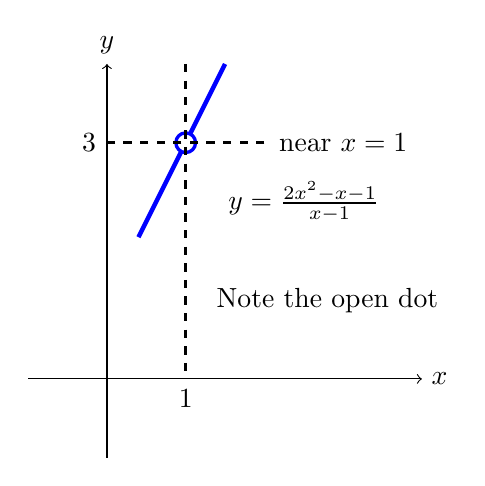
\begin{tikzpicture}[scale =1.0]
\draw[->] (-1,0) -- (4,0) node[right]{$x$};
\draw[->] (0,-1) -- (0,4) node[above]{$y$};
\draw[domain=0.4:0.95, smooth, variable=\x, blue, ultra thick] plot ({\x}, {(2*\x+1)});

\draw[blue, very thick]  (1,3) circle[radius=.125];

\draw[domain=1.05:1.5, smooth, variable=\x, blue, ultra thick] plot ({\x}, {(2*\x+1)});

\node at (2.5,2.25) {$y=\frac{2x^2-x-1}{x-1}$};
\node at (2.8,1) {Note the open dot};
\draw[black, very thick, dashed] (1,4)--(1,0)  node[below]{$1$};
\draw[black, very thick, dashed] (2,3)--(0,3) node[left]{$3$} ;
\node at (3,3) {near $x=1$};
\end{tikzpicture}
\caption{}
\label{fig:limitGraph}
\end{figure}
\end{multicols}
\begin{comment}
\begin{figure}[h]
\includegraphics[width=0.35\textwidth]{limits/limitGraph}
\caption{}
\label{fig:limitGraph}
\end{figure}
\end{comment}

\begin{comment}
%%%%%%%Example%%%%%%%%%%
%Example 4(a) from \cite{Hoffman} on page 81 including all three approaches (table, graph and algebra).
\begin{example}
Evaluate the following limit: \(\lim\limits_{x \to 0} \displaystyle \frac{x^2+5x+6}{x^2+3x+2}\)
    %%short answer
    \begin{sol}
    3
    \end{sol}
    %%solution
    \begin{solL}
    Let \(f(x)=\sqrt{25-x^2}\). So, $\lim\limits_{x \to -1} f(x)=f(4)=\sqrt{25-4^2}=3$.
    
    \end{solL}
    
\end{example}
\vspace{1.2 in}
\end{comment}
\begin{comment}
%%%%%%%Sub-Section%%%%%%%%%%%%
\subsection*{Some Techniques for Finding Limits using Formulas (Algebra Method)}
\begin{itemize}
    \item Limits of Some Very Nice Functions:  Substitution (see \cite{Hoffman}; pg.88).
    \item Limits of Polynomial and Rational Functions
    \item Limit of Other Combinations of Function (see \cite{Hoffman}; pg.88).
    \item Calculating a Limit When \(\frac{f(x)}{g(x)}\) has the indeterminate form \(\frac{0}{0}\) (\cite{openstax};page 164)
\end{itemize}
\end{comment}

%%The Limit Laws>Limits of Polynomial and Rational Functions>Theorem 2.6; pg. 162 from Openstax
\noindent \textbf{Finding Limits of Polynomial and Rational Functions by Substitution}\\
\noindent By now you have probably noticed that, in each of the previous examples, it has been the case that \(\lim\limits_{x \to a} f(x)=f(a)\) is not always true, but it does hold for all polynomials for any choice of a and for all rational functions at all values of a for which the rational function is defined.\\% Openstax; Limits of Polyonimial and Rational Functions;page 162

\begin{tcolorbox}[title = {Limits of Polynomial and Rational Functions}]

\begin{center}
\textbf{If} $P(x)$ and $Q(x)$ are \textbf{polynomials} and $a$ is any real number,\\
\textbf{then} \(\lim\limits_{x \to a} P(x)=P(a)\) and \(\lim\limits_{x \to a} \displaystyle\frac{P(x)}{Q(x)}=\displaystyle\frac{P(a)}{Q(a)}\) \textbf{if} \(\bm{Q(a)\ne 0}\)
\end{center}
In other words, we can calculate the limits of polynomials and rational functions by
substituting \underline{\emph{as long as the substitution does not result in a division by zero}}.
\end{tcolorbox}
%%%%%%%Example%%%%%%%%%%
%\noindent \textbf{Practice 2} from \cite{Hoffman}; page 88 and add finding the limit of a linear function. Address that the linear function is just a polynomial degree 1.
\vspace{-0.5cm}
\begin{example}
Evaluate the following limit: \(\lim\limits_{x \to 2} 5x^3-x^2+3\).
    %%short answer
    \begin{sol}
    39
    \end{sol}
    %%solution
    \begin{solL}
    ??
    
    \end{solL}
    
\end{example}
\vspace{0.6 in}
%\noindent \textbf{Practice 2} from \cite{Hoffman}; page 88 and add finding the limit of a linear function. Address that the linear function is just a polynomial degree 1.

\begin{example}
Evaluate the following limit: \(\lim\limits_{x \to 2} \displaystyle \frac{x^3-7x}{x^2+3x}\).
    %%short answer
    \begin{sol}
    $-\frac{3}{5}$
    \end{sol}
    %%solution
    \begin{solL}
    ??
    
    \end{solL}
    
\end{example}
\vspace{1.2 in}
\begin{comment}
%\noindent \textbf{Practice 2} from \cite{Hoffman}; page 88 and add finding the limit of a linear function. Address that the linear function is just a polynomial degree 1.
\begin{example}
Evaluate the following limit: \(\lim\limits_{x \to 2} \displaystyle \frac{x^2-2x}{x^2-x-2}\).
    %%short answer
    \begin{sol}
      $\frac{2}{3}$
    \end{sol}
    %%solution
    \begin{solL}
    ??
    
    \end{solL}
    
\end{example}
\vspace{0.6 in}
\end{comment}
\begin{example}
Evaluate the following limit: \(\lim\limits_{x \to 2} 4x+2\). \emph{Hint: A linear function is a polynomial degree 1}.
    %%short answer
    \begin{sol}
      10
    \end{sol}
    %%solution
    \begin{solL}
    ??
    
    \end{solL}
    
\end{example}
\newpage
\noindent For some functions, it is possible to calculate the limit as $x$ approaches a simply by substituting $x = a$ into the function and then evaluating $\dfrac{f(a)}{g(a)}$, but sometimes this method does not work since $\dfrac{f(a)}{g(a)}$ has an indeterminate form \(\left(ex.\ \displaystyle\frac{0}{0}, \displaystyle\frac{\infty}{\infty}, \displaystyle\frac{\infty}{0} \ etc. \right)\). These forms are common in calculus. In fact, the limit definition of the derivative which will be discussed in the next lesson is the limit of the indeterminate form of $\dfrac{0}{0}$.\\
%%%%Openstax Calculus Vol.I 2.3 The Limit Laws 165%%%%%%%%%%%%%%%%%
\begin{tcolorbox}[title = {Calculating a Limit When \(\displaystyle\frac{f(a)}{g(a)}\) has the indeterminate form of $\dfrac{0}{0}$}]
To find \(\lim\limits_{x \to a} \dfrac{f(x)}{g(x)}\) where \(f(a)=0\) and \(g(a)=0\), follow the steps below.
\begin{enumerate}[leftmargin=*]

\item Find an expression that is equal to \(\displaystyle\frac{f(x)}{g(x)}\) for all \(x\ne a\) over some interval containing \(a\). To do this, we may need to try one or more of the following steps:
\begin{enumerate}
    \item If \(f(x)\) and \(g(x)\) are polynomials in expanded form, we should factor each function and cancel out any common factors.
    
    \item If \(f(x)\) is polynomials in factored form and \(g(x)\) is a monomial, we should first expand \(f(x)\) and then simplify \(\displaystyle\frac{f(x)}{g(x)}\).
    
    \item If the numerator or denominator contains a difference involving a square root, we should try multiplying the numerator and denominator by the conjugate of the expression involving the square root.
    \item If \(\displaystyle\frac{f(x)}{g(x)}\) is a complex fraction, we begin by simplifying it.
\end{enumerate}
\item Find the limit by substitution and/or limit rules (see page \pageref{limitRules}).
\end{enumerate}

\end{tcolorbox}

\begin{comment}
\begin{itemize}
  
   \item Examples 3 from \cite{Hoffman} ; page 79
    \item Examples 2.17-2.20 from \cite{openstax}; pages 165-167.
    \item Example 2.5 (OpenStax; pg.138): Evaluate \(\lim\limits_{x \to 4} \displaystyle \frac{\sqrt{x}-2}{x-4}\) using a table of functional values\\\\
    \item Practice 2.4 (OpenStax; pg.139): Estimate \(\lim\limits_{x \to 1} \displaystyle \frac{\frac{1}{x}-1}{x-1}\)\\
\end{itemize}
\end{comment}
%%%%%%Example%%%%%%%%%%%%%
 %Example 4(b) from \cite{Hoffman} on page 81 including all three approaches (table, graph and algebra).
\begin{example}
Refer to Example \ref{ex1}. Algebraically, evaluate  \(\lim\limits_{x \to 1} f(x)\).

    %%short answer
    \begin{sol}
      3
    \end{sol}
    %%solution
    \begin{solL}
    ??
    
    \end{solL}
    
\end{example}
\vspace*{\stretch{1}}
%example 2.18 OpenStax Calculus Vol.I
\begin{example}
Algebraically, evaluate  \(\lim\limits_{x \to -1} \dfrac{\sqrt{x+2}-1}{x+1}\).

    %%short answer
    \begin{sol}
      \dfrac{1}{2}
    \end{sol}
    %%solution
    \begin{solL}
    ??
    
    \end{solL}
    
\end{example}
\vspace*{\stretch{1}}

\begin{example}
Given \(f(x)=x^2+3\), algebraically evaluate \(\lim\limits_{h \to 0} \dfrac{f(x+h)-f(x)}{h}\).
    %%short answer
    \begin{sol}
    2x
    \end{sol}
    %%solution
    \begin{solL}
    ??
    \end{solL}
    
\end{example}
\vspace*{\stretch{1}}

\newpage
\subsection*{Some Basic Limit Rules}\label{limitRules}
\begin{tcolorbox}[title = {Some Basic Limit Rules}]
For any real number $a$ and any constant $c$ where $\lim\limits_{x \to a}f(x)=L$ and $\lim\limits_{x \to a}g(x)=M$

\begin{equation}\label{eq:limitRule1}
\lim\limits_{x \to a}f(x)=f(a)
\end{equation}
\vspace{-0.5cm}
\begin{equation}\label{eq:limitRule2}
\lim\limits_{x \to a}c=c
\end{equation}
\vspace{-0.5cm}
\begin{equation}\label{eq:limitRule3}
\lim\limits_{x \to a}\left[f(x)+g(x)\right]=\lim\limits_{x \to a}f(x)+\lim\limits_{x \to a}g(x)=L+M
\end{equation}
\vspace{-0.5cm}
\begin{equation}\label{eq:limitRule4}
\lim\limits_{x \to a}\left[f(x)-g(x)\right]=\lim\limits_{x \to a}f(x)-\lim\limits_{x \to a}g(x)=L-M
\end{equation}
\vspace{-0.5cm}
\begin{equation}\label{eq:limitRule5}
\lim\limits_{x \to a}\dfrac{f(x)}{g(x)}=\dfrac{\lim\limits_{x \to a}f(x)}{\lim\limits_{x \to a}g(x)}=\dfrac{L}{m}\ \text{for} M\ne 0
\end{equation}

\end{tcolorbox}
%%%%%%%Examples%%%%%%
%\noindent \textbf{Example 1} of 'Limits of Other Combinations of Function' from  \cite{Hoffman} ; page 88.\\\\
\vspace{-0.5cm}
\begin{example}
Use the graph of $f(x)$ in Figure \ref{fig:exLimitCombinationFn} to evaluate the following limit:
\begin{multicols}{4}
\noindent (a) \(\lim\limits_{x \to 1} \{3+f(x)\}\) 
(b) \(\lim\limits_{x \to 1} \displaystyle{f(2+x)}\) 
(c) \(\lim\limits_{x \to 0}  \displaystyle{f(3-x)}\)
(d) \(\lim\limits_{x \to 2} \{f(x+1)-f(x)\}\)
\end{multicols}

    %%short answer
    \begin{sol}
     5; 1; 1;-2
    \end{sol}
    %%solution
    \begin{solL}
    ??
    
    \end{solL}
    
\end{example}

\begin{wrapfigure}[1]{l}{0.25\textwidth}
\begin{figure}[H]
\captionsetup[figure]{labelsep=space}
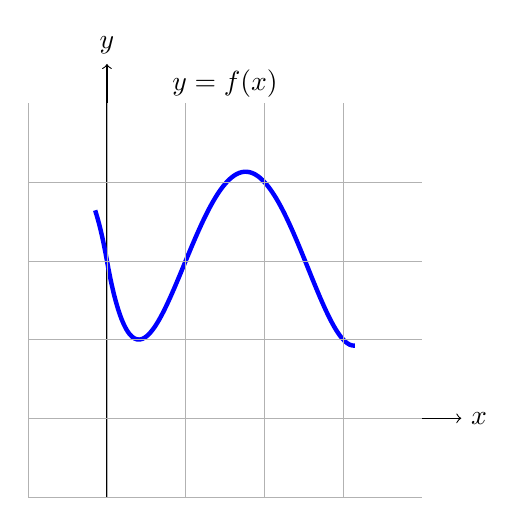
\begin{tikzpicture}[scale =1.0]
\draw[->] (-1,0) -- (4.5,0) node[right]{$x$};
\draw[->] (0,-1) -- (0,4.5) node[above]{$y$};
\node at (1.5,4.25) {$y=f(x)$};
\draw[domain=-0.15:3.15, smooth, variable=\x, blue, ultra thick, samples=100] plot ({\x}, {(5*\x^4)/8 - (53*\x^3)/12 + (75*\x^2)/8 - (67*\x)/12 + 2});
\foreach \x in {-1,...,3}
	{\draw[ line width=0.2pt, black!30!white] (\x,-1) grid (\x,4);
	 \draw[ line width=0.2pt, black!30!white] (-1,\x) grid (4,\x);}
\end{tikzpicture}
\caption{}
\label{fig:exLimitCombinationFn}
\end{figure}
\end{wrapfigure} 

\begin{comment} 
\begin{wrapfigure}[1]{l}{0.25\textwidth}
    \includegraphics[width=\textwidth]{limits/exLimitCombinationFn}
    \caption{}
    \label{fig:exLimitCombinationFn}
\end{wrapfigure}
\end{comment}

\hfill


\newpage

\subsection*{One-Sided Limits}
\begin{comment}
\begin{itemize}
    \item One-Sided Limits at the bottom of page 143 of \cite{openstax} text.
    \item One-Sided Limits; page 82 of \cite{Hoffman} text.
\end{itemize}
\end{comment}
%%%Hoffman; page 82%%%%%%%
Sometimes, what happens to us at a place depends on the direction we use to
approach that place. If we approach Niagara Falls from the upstream side, then we
will be 182 feet higher and have different worries than if we approach from the
downstream side. Similarly, the values of a function near a point may depend on the
direction we use to approach that point.
\begin{tcolorbox}[title = {Definition of Left and Right Limits}]
The \textbf{left limit} as $x$ approaches $c$ of $f(x)$ is $L$ if the values of $f(x)$ get as close to $L$ as we want when $x$ is very close to and \emph{left of c} (or $x<c$) 
\vspace{-0.25cm}
\begin{equation}\label{eq:leftLimitDef}
\lim\limits_{x \to c^-}f(x)=L
\end{equation}
The \textbf{right limit} as $x$ approaches $c$ of $f(x)$ is $L$ if the values of $f(x)$ get as close to $L$ as we want when $x$ is very close to and \emph{right of c} (or $x>c$) 
\vspace{-0.25cm}
\begin{equation}\label{eq:limitRule2}
\lim\limits_{x \to c^+}f(x)=L
\end{equation}

\end{tcolorbox}
%Example 2.8 (OpenStax; pg.144)\\
\begin{example}\label{exOneSidedLimit}
Given the function $f(x)$ below, 
\begin{align*}
f(x) = \left\{ \begin{array}{cc} 
                x+1 & \hspace{2mm} \textrm{if} \quad x<2 \\
                x^2-4 & \hspace{2mm} \textrm{if} \quad x\ge 2 \\
                \end{array} \right.
\end{align*}
evaluate each of the following limits using Table \ref{table:limitTable3} and the given graph of $f(x)$ (Figure \ref{fig:oneSidedLimit}). Explain how you reach your answers.
\begin{multicols}{2}

\begin{enumerate}[leftmargin=*]
   \item $\lim\limits_{x \to 2^-}f(x)$
    \item $\lim\limits_{x \to 2^+}f(x)$
\end{enumerate}

\end{multicols}
    %%short answer
    \begin{sol}
      3;0
    \end{sol}
    %%solution
    \begin{solL}
    ??
    
    \end{solL}
    
\end{example}

\begin{multicols}{2}

\begin{table}[H]
%\renewcommand{\thetable}{1.2}
\caption{}
\label{table:limitTable3}
\begin{center}
\begin{tabular}{|l|l|l|l|}
\hline
$x$ & $f(x)=x+1$ & $x$ & $f(x)=x^2-4$ \\
\hline
1.9	&	2.9 & 2.1 & 0.41\\
\hline
1.99	&	2.99 & 2.01 & 0.0401\\
\hline
1.999	&	2.999 & 2.001 & 0.004001\\
\hline
1.9999	&	2.9999 & 2.0001 & 0.00040001\\
\hline
1.99999	&	2.99999 & 2.00001 & 0.0000400001\\
\hline
\end{tabular}
\end{center}
\end{table}

\begin{figure}[H]

\captionsetup[figure]{labelsep=space}
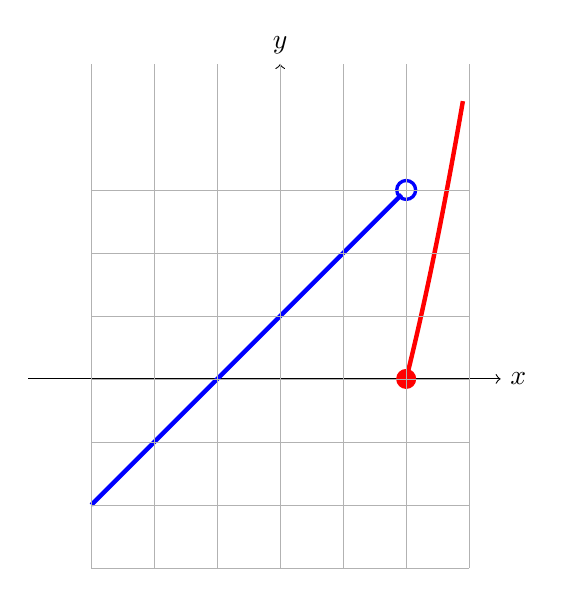
\begin{tikzpicture}[scale =0.8]
\draw[->] (-4,0) -- (3.5,0) node[right]{$x$};
\draw[->] (0,-3) -- (0,5) node[above]{$y$};

\draw[domain=-3:1.925, smooth, variable=\x, blue, ultra thick] plot ({\x}, {(\x+1)});

\draw[blue, very thick]  (2,3) circle[radius=.15];

\draw[domain=2.035:2.9, smooth, variable=\x, red, ultra thick] plot ({\x}, {(\x^2-4)});

\filldraw[red]  (2,0) circle[radius=.15];

\foreach \x in {-3,...,3}
	{\draw[ line width=0.2pt, black!30!white] (\x,-3) grid (\x,5);
	 \draw[ line width=0.2pt, black!30!white] (-3,\x) grid (3,\x);}
\end{tikzpicture}
\caption{}
\label{fig:oneSidedLimit}
\end{figure}

\end{multicols}


%%%%%%%%%%%%%%%%%%%%%%%%%%%%%%
\begin{comment}
\vspace{-0.5cm}
\begin{figure}[h]%
    \centering
    \subfloat[]{{\includegraphics[width=8cm]{limits/oneSidedLimitTable} }}%
    \qquad
    \subfloat[]{{\includegraphics[width=5cm]{limits/oneSidedLimitGraph} }}%
    \caption{}%
    \label{fig:oneSidedLimit}%
\end{figure}
\vspace{-0.5cm}
\end{comment}
%%%%%%%%%%%%%%%%%%%%%%%%%%%
%Examples 3 from Dave's handout
\begin{example}
Evaluate the following limit: \(\lim\limits_{x \to 0^+} \left(\displaystyle \frac{1}{x} +2\right)\).
    %%short answer
    \begin{sol}
    $\infty$
    \end{sol}
    %%solution
    \begin{solL}
    ??
    \end{solL}
\end{example}
\vspace{1.2 in}

\newpage
\subsection*{The Existence of a Limit}
%%OpenStax;One-Sided Limits; pg. 145
Let us now consider the relationship between the limit of a function at a point versus the limits from the right and left at that point. It seems clear that if the limit from the right and the limit from the left have a common value, then that common value is the limit of the function at that point. Similarly, if the limit from the left and the limit from the right take on different values, the limit of the function does not exist. These conclusions are summarized in the box below:\\
%Hoffman;page 83
\begin{tcolorbox}[title = {One-Sided Limit Theorem:}]
\begin{center}
$\lim\limits_{x \to c}f(x)=L$ if and only if $\lim\limits_{x \to c^-}f(x)=\lim\limits_{x \to c^+}f(x)=L$
\end{center}
\end{tcolorbox}

\begin{tcolorbox}[title = {Corollary:}]
\begin{center}
If $\lim\limits_{x \to c^-}f(x)\ne \lim\limits_{x \to c^+}f(x)$, then $\lim\limits_{x \to c}f(x)$ does not exist.
\end{center}
\end{tcolorbox}


%%%Examples%%%

\begin{example}
Refer to the function $f(x)$ in Example \ref{exOneSidedLimit}, does $\lim\limits_{x \to 2}f(x)$ exist? Explain your reasoning.
%%short answer
    \begin{sol}
    No.
    \end{sol}
    %%solution
    \begin{solL}
    No because $\lim\limits_{x \to -2}f(x) \ne \lim\limits_{x \to 2}f(x)$.
    
    \end{solL}
\end{example}
\vspace{1.7in}
%Examples 6 from Dave's handout
\begin{example}
Evaluate the following limit: \(\lim\limits_{x \to 2} \left(\displaystyle \frac{x^2+2x}{x^2-4}\right)\). If it does not exist, explain your reasoning.
    %%short answer
    \begin{sol}
    No limit exists.
    \end{sol}
    %%solution
    \begin{solL}
    ??
    \end{solL}
\end{example}
\vspace{1.7in}
\begin{comment}
%1111111111111111
\begin{example}
Evaluate the following limit: \(\lim\limits_{x \to 4}  \sqrt{25-x^2}\)
    %%short answer
    \begin{sol}
    3
    \end{sol}
    %%solution
    \begin{solL}
    Let \(f(x)=\sqrt{25-x^2}\). So, $\lim\limits_{x \to -1} f(x)=f(4)=\sqrt{25-4^2}=3$.
    
    \end{solL}
    
\end{example}

\vspace{1.2 in}

%222222222222222

\begin{example}
Evaluate the following limit: \(\lim\limits_{x \to -1} \displaystyle\frac{2x}{x^2-2}\)
    %%short answer
    \begin{sol}
    2
    \end{sol}
    %%solution
    \begin{solL}
    solution
    \end{solL}
    
\end{example}

\vspace{1.2 in}

%333333333333333

\begin{example}
Evaluate the following limit: \( \lim\limits_{x \to 0} \displaystyle\left(\frac{1}{x}+2\right)\)
    %%short answer
    \begin{sol}
    \small No limit exists.
    \end{sol}
    %%solution
    \begin{solL}
    solution
    \end{solL}

\end{example}

\vspace{1.2 in}

%4444444444444

\begin{example}
Evaluate the following limit: \( \lim\limits_{x \to 0} \displaystyle\left(\frac{x^2-4x}{x}\right)\) (check the graph)
    %%short answer
    \begin{sol}
    -4
    \end{sol}
    %%solution
    \begin{solL}
    solution
    \end{solL}

\end{example}

\vspace{1.3 in}

%5555555555

\begin{example}
Evaluate the following limit: \( \lim\limits_{x \to 2} \displaystyle\left(\frac{x^2-2x}{x^2-4}\right)\) 
    %%short answer
    \begin{sol}
    0.5
    \end{sol}
    %%solution
    \begin{solL}
    solution
    \end{solL}

\end{example}

\newpage
%666666666666

\begin{example}
Evaluate the following limit: \( \lim\limits_{x \to 2^+} \displaystyle\left(\frac{x^2+2x}{x^2-4}\right)\) 
    %%short answer
    \begin{sol}
   \small No limit exists.
    \end{sol}
    %%solution
    \begin{solL}
    solution
    \end{solL}

\end{example}

\vspace{1.1 in}

%7777777777777

\begin{example}
Evaluate the following limit: \( \lim\limits_{x \to \infty} \displaystyle\left(\frac{1}{x^2-4}\right)\) 
    %%short answer
    \begin{sol}
    0
    \end{sol}
    %%solution
    \begin{solL}
    solution
    \end{solL}

\end{example}

\vspace{1 in}

%88888888888888

\begin{example}
Evaluate the following limit: \( \lim\limits_{x \to \infty} \displaystyle\left(\frac{2x^2+4x}{x^2-4}\right)\) 
    %%short answer
    \begin{sol}
    2
    \end{sol}
    %%solution
    \begin{solL}
    solution
    \end{solL}

\end{example}

\vspace{1 in}

%9999999999999999

\begin{example}
Evaluate the following limit: \( \lim\limits_{x \to \infty} \displaystyle\left(\frac{1000x}{x^2-2000}\right)\) 
    %%short answer
    \begin{sol}
    0
    \end{sol}
    %%solution
    \begin{solL}
    solution
    \end{solL}

\end{example}

\vspace{1 in}

%101010101010

\begin{example}
Evaluate the following limit: \( \lim\limits_{x \to \infty} \displaystyle\left(\frac{1}{x}-5\right)\) 
    %%short answer
    \begin{sol}
    -5
    \end{sol}
    %%solution
    \begin{solL}
    solution
    \end{solL}

\end{example}

\vspace{1 in}
\end{comment}
\Closesolutionfile{ans}
\Closesolutionfile{ansL}
%%%Short Answers to Examples%%%
\subsection*{Short Answers}
\begin{multicols}{4}
\input{ans1}
\end{multicols}
\newpage


